 %	Skriv folgende ind som en custom Quick Build (F1)
%pdflatex -interaction=nonstopmode %.tex|bibtex %|pdflatex -interaction=nonstopmode %.tex|pdflatex -interaction=nonstopmode %.tex

\input{layout/preamble_P4_draft.tex}
\newenvironment{boenumerate}
  {\begin{enumerate}\renewcommand\labelenumi{\textbf\theenumi}}
  {\end{enumerate}}

\begin{document}
	
	\lstset{frameround=tttt, escapeinside={\%}{\%}}
	
	%\title{GIRAF - Admin}
%\author{By: Group SW601F12}
%\date{\emph{May 2013}}
%\maketitle
%\newpage

\thispagestyle{empty}
\begin{flushright}
\vspace{3cm}

\phantom{hul}

\phantom{hul}

\phantom{hul}

\textsl{\Huge Parental Control - In Smart Home} \\ \vspace{1cm}

\rule{13cm}{3mm} \\ \vspace{1.5cm}
\vspace{1cm}

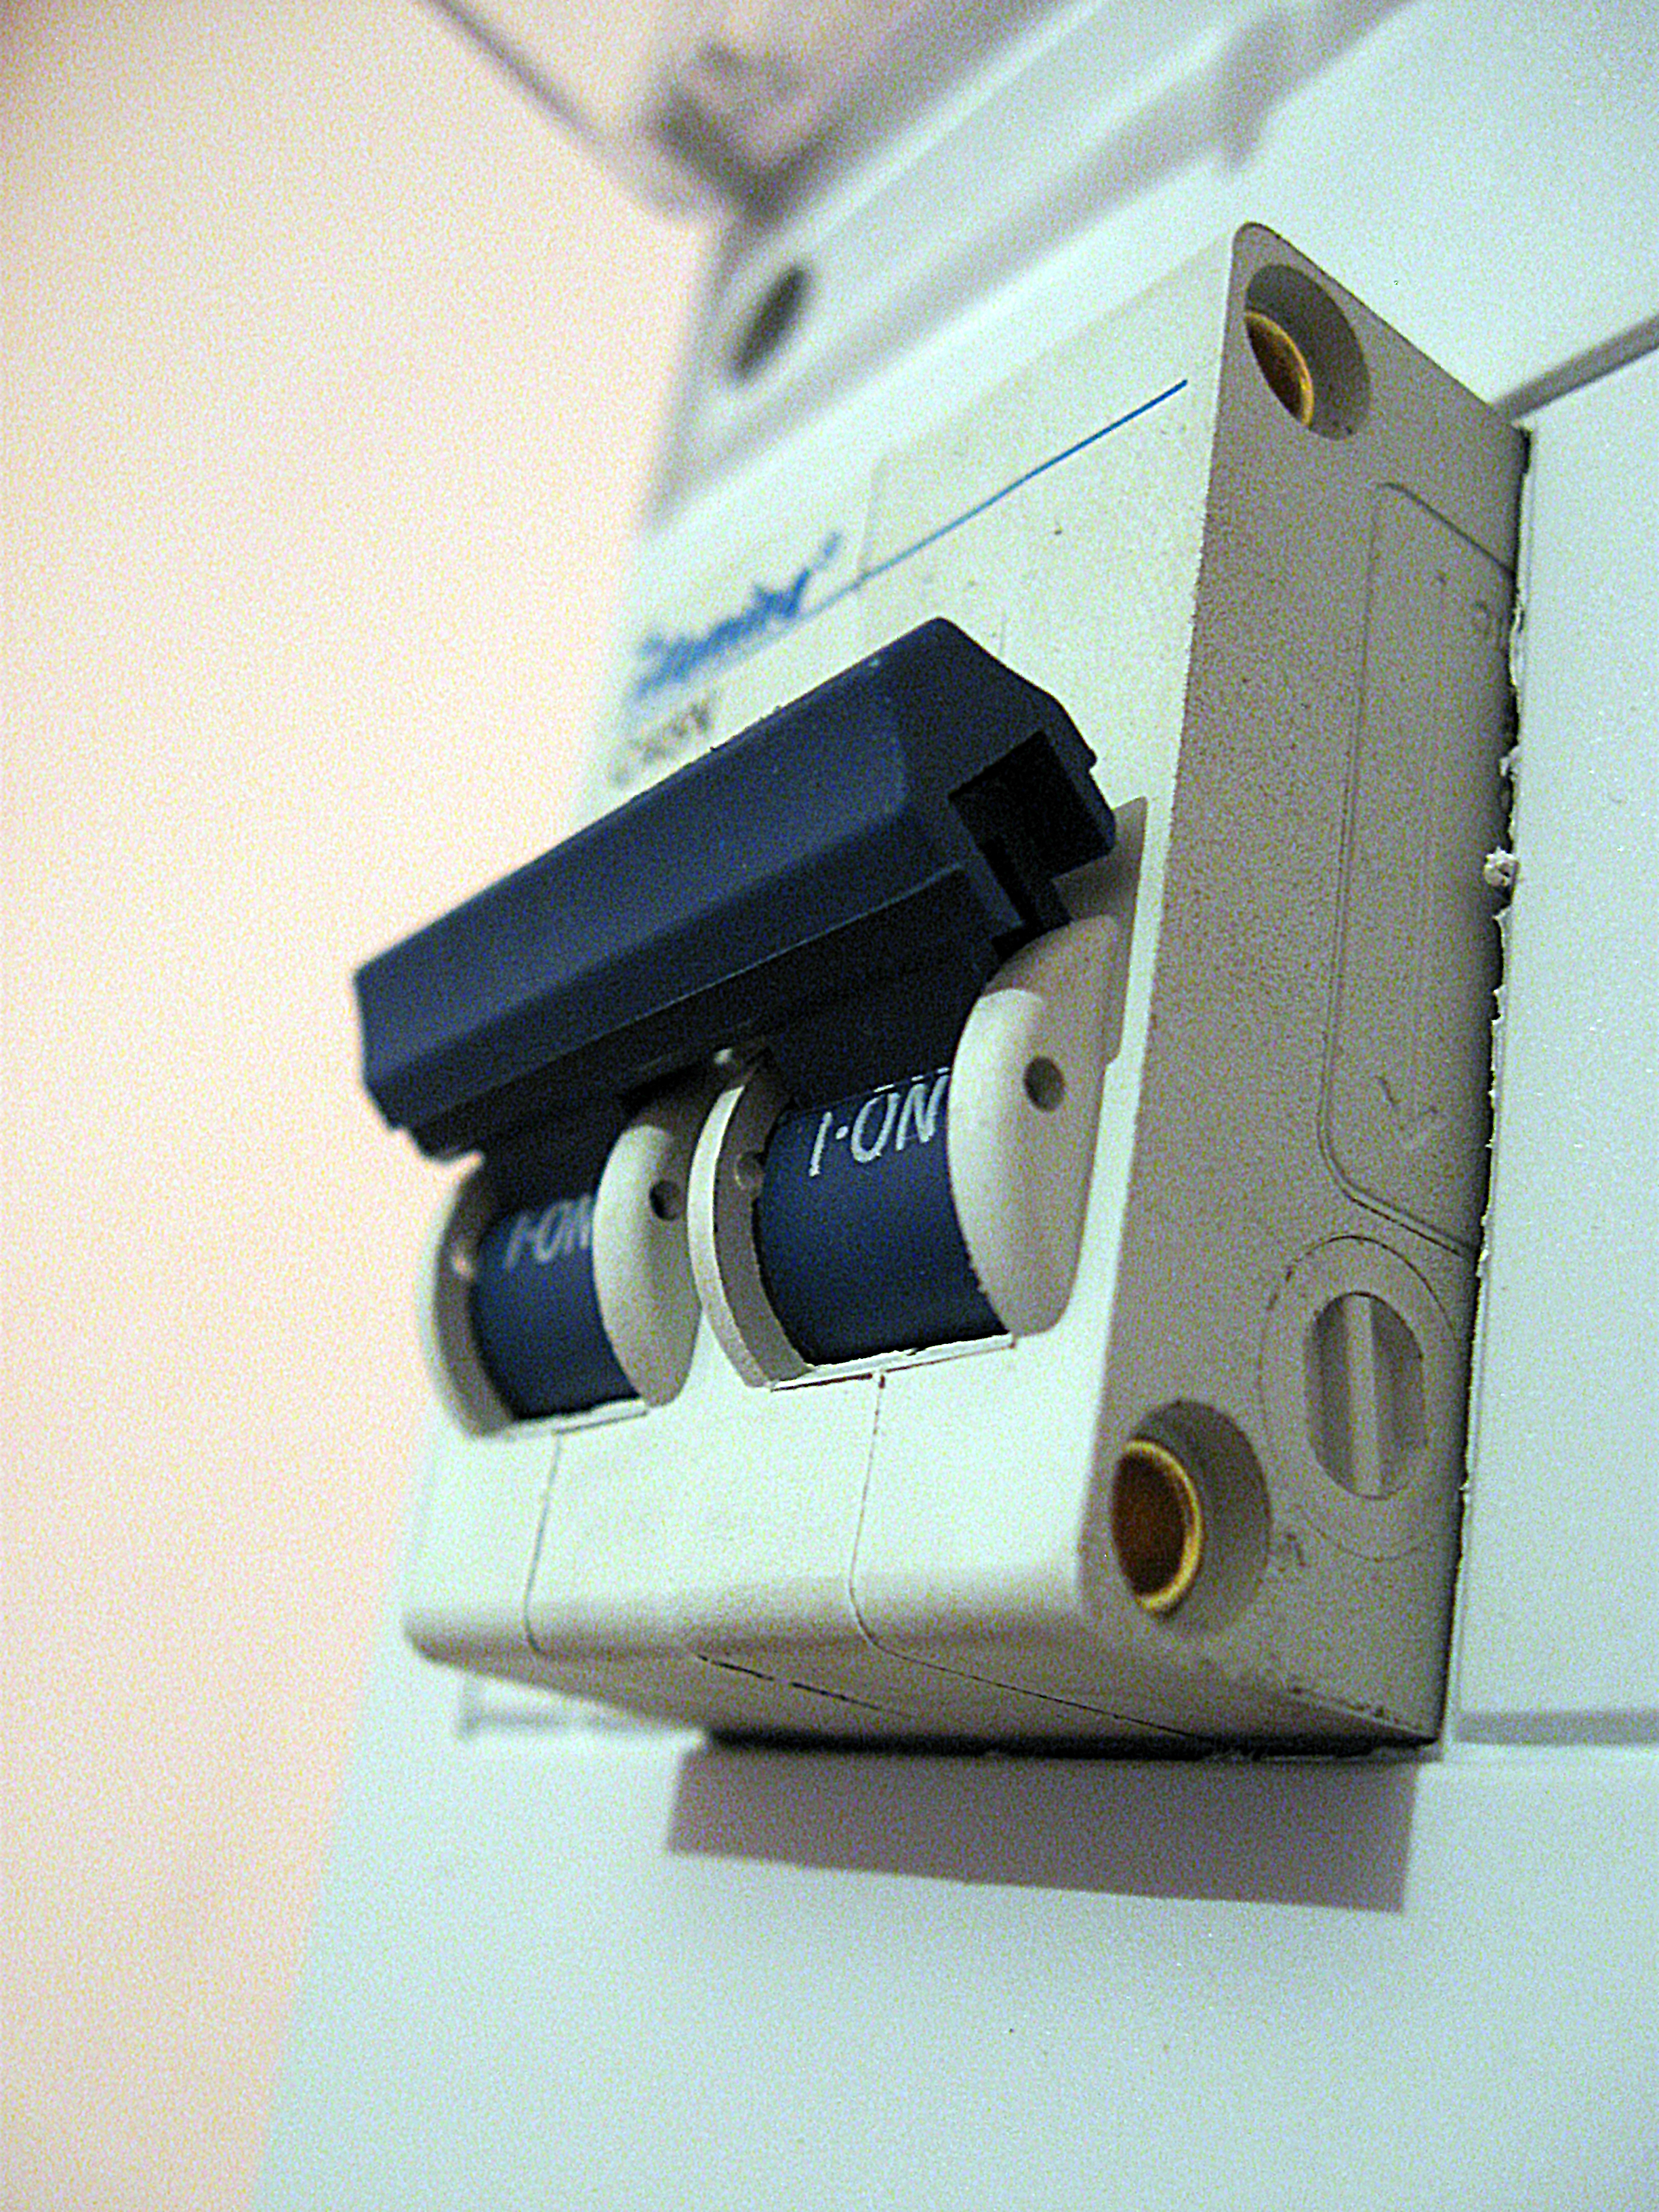
\includegraphics[width=0.75\textwidth, height=0.45\textheight]{images/HFIswitch.jpg}


\vspace{1.5cm} 
\textsc{\Large SW7 Projekt \\
Group SW701E13 \\
Department of Computer Science\\
Aalborg University\\
December 20$^{th}$ 2013\\}
\end{flushright}

	\addtocounter{page}{1}
	\input{layout/emptypage.tex}
%	\setcounter{page}{2}
	\thispagestyle{empty}
\begin{titlepage}
	\addcontentsline{toc}{chapter}{Title Page}
	\setcounter{page}{3}
\begin{nopagebreak}
{\samepage 
\begin{tabular}{r}
\parbox{\textwidth}{  \raisebox{-14mm} {\includegraphics[height=3.0cm]{images/aau-stud-logo.pdf}}
\hfill \parbox{4.9cm}{\begin{tabular}{l}
{\sf\small \textbf{Department of Computer Science}}\\
{\sf\small  \textbf{Aalborg University}} \\
{\sf\small Selma Lagerl\"{o}fs Vej 300} \\
{\sf\small Telephone: +45 9940 9940} \\
{\sf\small Telefax:   +45 9940 9798} \\
{\sf\small http://cs.aau.dk}
\end{tabular}}}
\\
\end{tabular}
\vspace{-12pt}
\begin{tabular}{cc}
\parbox{7cm}{
\begin{description}

\item {\bf Title:} 

Parental Control - In Smart Home

\item {\bf Theme:} 

Internet Technology

\end{description}

\parbox{8cm}{

\begin{description}
\item {\bf Project period:}\\
   P7, Autumn Term 2013\\
  \hspace{4cm}
\item {\bf Project group:}\\
  SW701E13\\
  \hspace{4cm}
\item {\bf Participants:}\\
Jens M. Lauridsen\\
Johan Sørensen \\
Lars Chr. Pedersen\\
Tommy Knudsen\\
Lisbeth Nielsen\\
Jakob Jørgensen
  \hspace{2cm}
\item {\bf Supervisor:}\\
Hua Lu
\end{description}
}
\begin{description}
\item {\bf Circulation:} 8
\item {\bf Page count:} \pageref{LastPage}
\item {\bf Appendix count and type:} 4, Rules first design, Light Table, RFID Output, Test Suite
\item {\bf Finished on} December 20$^{th}$ 2013
\end{description}
\vfill } &
\parbox{7cm}{
  \vspace{.15cm}
  \hfill 
  \begin{tabular}{l}
  {\bf Synopsis:}\bigskip \\
  \fbox{
    \parbox{6.5cm}{\bigskip
     {\vfill{\small This report documents the development of a system which aims to decrease children's media consumption. 
The report is developed by a 7th semester Software engineering group.
The system consists of a website for setting up the system, a database to store the settings, an Arduino with an RFID reader to identify users and restrict usage of media, and a daemon to automate point giving.
A combination of different programming languages was used both for the front- and back-end, a list can be found in the end of the report.
The prototype has been completed and is close to a state, valid for real life testing.
     \bigskip}}
     }}
   \end{tabular}}
\end{tabular}}
\\ \\ \\ \\
\noindent{\footnotesize\emph{The report content is freely available, but publication (with source), only after agreement with the authors.}}
\end{nopagebreak}
\end{titlepage}
	\input{layout/emptypage.tex}
	\chapter*{Preface}
\label{chap:preface}
%Preface goes here...
This report is written by six students from the Department of Computer Science at Aalborg University, and is a project under the subject ``Internet of Things''. The six students are studying as Software Engineers at their 7th semester.\\
\\
This report serves as a suggestion of how to moderate children's increasing use of media.\\
\\
Included with this report, there is a CD containing the project's Git repository. Which contains the report, source code of the system as well as the graphic assets used in the project.\\
\\
The group would like to personally thank:\\
Hua Lu our counselor.
%Ulrik Nyman for great input and support during the project.\\
%Mette Als for her patience and valuable input into the designing of the system.\\

	\input{layout/emptypage.tex}
%	\setcounter{page}{4}
	\input{layout/signatures.tex}
	\input{layout/emptypage.tex}
%	\setcounter{page}{6}
	\tableofcontents	
	\addcontentsline{toc}{chapter}{Contents}
	\newpage
	
	%\part{Design}
	

	
	% Part Analysis
	\part{Analysis}
	\chapter{Project Focus}
This report is centered about Parental Control (PC) in Smart Home (SH). This chapter will explain what PC and SH is, as well as explorer a field of different possibilities and narrow the possibilities down to a reasonable amount of goals for this project.

%What is smart home
\section{Smart Home}
A Smart Home can refer to multiple forms of improvement on a home. Most commonly is home automation, environment friendly improvements and power saving improvements. In this report we will only regard Smart Home in relation to home automation, however environment friendly- and power saving improvements, sometimes also springs out of home automation. For example if you automate the washing machine to start at a certain hour of the day, it will both be convenient as well as power saving.\\
\\
But a Smart Home, can be much more. Different examples of implementable features is as follows:

\begin{itemize}
	\item Automated security
	\item Music systems
	\item Theater systems
	\item Voice commands
	\item Automatic ordering of groceries
	\item Delayed start on an oven
	\item Automated coffee machines
	\item Light control
	\item Power control on leaving home
	\item And much more
\end{itemize}

This report is about a less common feature of a Smart Home. It is about Parental Control, a concept explained in \ref{parentalControl}.

%What is parental control
\section{Parental Control}
\label{parentalControl}
Parental Control (PC) is a concept most people know from their TV at home or computers. A concept used mainly by parents to protect their children from fx. internet sites with adult content or TV channels of the same kind.\\
But in a Smart Home, this concept could be taken even further. Many electronic devises does not implement a PC feature, and some of those which does, does not allow to block all content.\\
We want to create a system that could help parents manage their children's time. We want to do this in order to improve the well being of children. Studies show that children of the newer ages are sitting indoors, more and more.\citep{childrenAndNature}\citep{leaveNoChildInside}\\
These studies also tell how staying inside both limits the child’s imagination and is a factor for stress. It has also been linked to an increase in likelihood of these children having ADHD.\\
\\
What this project is aiming at is to create a system that would allow the parents to both, help manage their children's time, as well as encourage them to go outside and play.\\
In order for this to succeed, the implementation must offer this control set, without becoming too much of a bother for both the parents and the children it impacts. We do not want to restrict and limit, but rather organize and encourage. - This effectively means, the system can not impose a too long addition to the start up of the restricted devices and the system must implement a feature for the children to earn more time for the restricted devices. These requirements will be gone into further details at a later point REF...

%Write about the brainstorm we did
\section{Potential of Parental Control}
In order to determine the potential for the Parental Control system, a brainstorm was made, to visualize the ideas and couplings that could be made with an existing Smart Home implementation. For this brainstorm we took the base concept of a Smart Home as introduced by Mi Casa Verde\citep{micasaverde}.


\begin{figure}[htbp]
	\centering
		\includegraphics[width=1.00\textwidth]{images/BrainStorm.png}
	\caption{Brainstorm over Parental Control}
	\label{fig:BrainStorm}
\end{figure}

%Explain each point of the Brainstorm, atleast the Green ones, also explain the color codes.
In figure \ref{fig:BrainStorm} is seen 3 different colors. Red is our starting point. Green is our direct sub-points and yellow is our indirect sub-points.\\
Next is a walkthrough of each of the direct sub-points.\\
\subsection{Chores}
\subsection{Rules}
\subsection{Calendar Integration}
\subsection{App. Integration}
\subsection{Computer}
\subsection{Noise Control}
\subsection{Baby Control}
\subsection{Food Control}
\subsection{Alternative ID and Security}


%Narrow down the area we want to covor
%Specify what must be done, in order for it to succed
	%	Who is the target group?
\chapter{The Children are Suffering}
In this chapter the target group is stated and it is explained why the target group would want to buy such a system.
 
\section{The Target Group}
This parental control system in a smart house is targeted at parents to children who are between 4 and 14.
We find the parents of children in the age group 0-3 to be less important since the children are too young to use the system.
Parent with children that are 15 or more are also less important because at that time the child might have bought his/hers own 
computer or television where the system should not be applied. Also the child would need the computer more for homework.  
    

\section{Children's Increased Media Usage}

There have been made many surveys that measure how much screen time children use on computers, television and console. These surveys 
have been made in several western countries, and their result typically indicates that children uses more 
time in front of the screen than either previous years or the recommended two hours. 
Even though this is general for many countries we only focus on the Danish marked and the Danish children.


%http://www.commonsensemedia.org/sites/default/files/research/zerotoeightfinal2011.pdf usa timer per day 3:46 children 5-8
%http://politiken.dk/tjek/forbrug/familieliv/ECE1779536/boern-bruger-syv-timer-daglig-foran-en-skaerm/ dk, 2,5 children 5-7
%http://www.biomedcentral.com/1471-2458/13/684 finland children 4th-6th grade (0:59 tv and 1:17 computer)

\subsection{Danish Children's media usage}
In 2012 a survey was made by TNS Gallup, where they looked into the 5-16 years old children's time usage of television, internet, computer games 
and console game. The average total time of the result can be found in table \ref{tab:Gallup2012screentime}. One point of critics of 
this survey is that it do not take into account that the children can use multiple media at the same time, so the actual number 
should be smaller. However, it can still be concluded from these results that even if most of the children uses two medias at a time
the exceed the recommended 2 hours per day. It can also be concluded that the time spend on the medias increases during the weekends and 
with age.

%cite: http://politiken.dk/tjek/forbrug/familieliv/ECE1779536/boern-bruger-syv-timer-daglig-foran-en-skaerm/

\begin{table}
\begin{center}
  \begin{tabular}{ | l | c | c | c | c || r | }
    \hline
				& 5-7 years & 8-10 years & 11-13 years & 14-16 years & In all\\ \hline
    Weekday 	&  		    &  			 &  		   &   			 & \\ 
	total time:  &	3:12	& 4:29		 &  6:13	   &  7:26		 & 5:23  \\ \hline
	Weekend &  &  &  &   & \\
	total time: &  	5:02	&  6:32		&  8:5		   &	9:15	& 7:17 \\ \hline
    \hline
  \end{tabular}
  \label{tab:Gallup2012screentime}
\end{center}
\end{table}

Seen from the general population and the states point of view this is a big problem because of the negative consequences that will follow 
too much media usage. 

\subsection{Consequences of Media Usage}
Two of the more common consequences of the children using the computer, console and television too much, is increasingly experience sleep disruptions 
and lack of physical exercise. Both of them also can lead to reducing in children's learning ability and other consequences which will be 
explained in the following sections.

 
\subsubsection*{Increasingly experiences sleep disruptions}
The child can experience disruption in his/hers sleep pattern. Typically the child that has media in his/hers room less that a child who do not. 
But also the usages of media have been proven to have an effect on the sleeping pattern. The sleep disruption can be more in form of too late bedtime
or disruption during sleep.
%cite http://www.sciencedaily.com/releases/2013/07/130725202325.htm 

The sleep disruptions can also lead to decreasing ability in visual and verbal memorizing which also have an effect on the
concentration difficulties in school. If the sleep disruption occurs too often then the child's health can be effected.
%cite http://pediatrics.aappublications.org/content/120/5/978.long



\subsubsection*{Lack of physical exercise}
The more the child is in front of a screen the less time is used on physical activities such as playing with other children, participating 
in sports or other recreational activities. Children in the age 5-17 years old are supposed to be physically active in an hour per day 
according to the Danish Board of Health. However, $2/3$ of the children do not meet this requirement and one of the reasons are 
the increased media usage.
%cite http://www.dr.dk/Nyheder/Indland/2013/09/29/235953.htm
This can also lead to serious health problems like obesity, diabetes and again concentration difficulties.  \\\\


Since too much media consumption is generally bad for the child it is important to understand why the parent do not control their media usage more, 
which is focused on in the next section.


\section{Parental Control - Ability and Tools} %senere overvej titlen

Generally weekdays of the parents are busy due to both parent's job, daily house work, and the children. However, the child has typically 
the school, maybe after-school care and recreational activities. Depending on the age of the child he/she maybe alone home in several hours 
before the parents get home. This is a time were the parents have no control of whether the child is using the television, console or computer. 
When the parents are at home the child might still be allowed to use the medias to much if the parents do or cannot keep track of their children's 
media usage.

The media rules and enforcement of them is probably different for each family, but something similar for the parents are the available tools to help 
them controlling the media usage. It should also be studied whether the parents feel they have the necessary tool to keep the children from
watching television and playing computer or console game.   

 
\subsection{our interviews}

more to come

	\chapter{Problem Statement}
As the prevues chapter explained, children's increase in media usage is becoming a problem. This is a problem we want to solve by the usage of modern technology, internet applications and physical recognition of users.\\
In this chapter a formal definition of the problem is written together with an emphasis on what challenges this problem rises.\\


\begin{verse}
\textit{Parents are not able of helping their children administer their IT/TV consumption.\\
This results in their children getting a lessened learning ability, a bad sleeping pattern and a higher risk of type 2 diabetes.\\
How can hardware identification and webservices give parents the tools to help their children manage their media consumption?}
	\begin{itemize}
		\item How do we identify unique users in a subtle and child friendly way.
		\item How do we enforce restrictions on media devices.
		\item How do we facilitate concepts as rules, permissions and chores without parents interaction.
	\end{itemize}
\end{verse}


With this formal statement of the problem in mind, the next chapter goes into detail of how we intend to solve these challenges.

%English: Parents are not able of helping their children administer their IT/TV consumption.
%This results in their kids getting a lessened learning ability, a bad sleeping pattern and more.
%How can smart home technology give parents the tools they need to help their children administer their IT/TV consumption?

%Edited version:
%How can hardware identification and webservices give parents the tools to help their children manage their media consumption. 
%(Childrens media consumptions is increasing, giving higher risks of type 2 diabetes.
	\chapter{Languages}
\label{chp:languages}
This chapter will explain which programming languages are used in this project. Why they are used and in some cases compare them to other solutions.\\
\subsection*{Front-end}
\label{sec:frontend} % INSERT CORRECT LINKS
HTML, CSS and JS will be used to develop the interface both for desktop and mobile devices. This selection is due to the fact that websites have no real alternatives. This project will not focus on developing for older web browsers hence it will be written in entirely HTML5 without regards to it not working in older browsers such as IE6.

\subsection*{Web-server}
\label{sec:webserver} % INSERT CORRECT LINKS
On the web-server there is the option to use a lot of different languages for implementing the back-end. To name a few: Java Servlets, ASP.NET, PHP, Ruby and Python. As the intention is that the software produced in this project is built on Open Source technologies and software. ASP.NET will not be considered any further even though mod\_ mono and other open source implementations exist simply as these do not offer the complete set of API available. When talking PHP vs Ruby and Python it generally is a tie in . But the ease with which one can set-up a test development on ones localhost is is big plus for PHP. Performance wise it depends heavenly on which type of application is run. Benchmarks shows in different favours. PHP and Java Servlets both have god and bad reputation depending on what area is looked into. The same is true for performance where there are reports showing in the favour of both. Some will argue that general code security is better in Servlets than in PHP while others will argue that it is completely the opposite that is the truth. \\
As the field is under constant development. One version of one of the systems might be far better performance wise but it still depends on what it is used for. The selection comes from what the group has of prior knowledge and experience and hence the selection is PHP as this is where the group feels most comfortable.


\subsection*{Arduino}
\label{sec:arduino} % INSERT CORRECT LINKS
The main programming languages used when programming for Arduino is C \& C++. This is therefore selected for the project and it enables the direct use of shields that are needed for the network and NFC communication. 

\subsection*{Back-end}
\label{sec:backend} 
The back-end of the system that communicates directly with the Arduino and in long term other devices can be designed in a number of different languages. This including PHP. The choice is therefore straight forward as the complete server side system then can run completely in PHP and no extra software is needed.

\subsection*{Language Support}
\label{sec:langSupport}
Localization is something that when designing a system is easy to take into account. But when the system is developed and near completion it can be difficult to implement. Therefore this will be taken into account from the start and in such a way that it supports most common languages.

\subsection*{Folder Structure}
\label{sec:folderStructure}
When designing a system which is supposed to come with a high maintainability it is important to design a usable folder structure. The folder structure of this project can be seen in figure \ref{fig:folderStructure}.\\
\\

\begin{figure}[htbp]
        \centering
                \includegraphics[width=0.25\textwidth]{images/folderStructure.png}
        \caption{The Code Folder Structure}
        \label{fig:folderStructure}
\end{figure}

\noindent{\textbf{web:} This is the main directory for the web interface.}\\
\\
\textbf{backend:} This is the main directory for the back end of the system.\\
\\
\textbf{api:} Is intended to contain API which are not JavaScript or PHP code.\\
\\
\textbf{assets:} Contains every asset in the system. Images, JavaScript, sound, fonts, CSS and language files.\\
\\
\textbf{assets - css:} Contains the CSS files for the system.\\
\\
\textbf{assets - fonts:} Contains special fonts for the system.\\
\\
\textbf{assets - ico:} Contains the icon files for the system.\\
\\
\textbf{assets - img:} Contains the static image resources for the system.\\
\\
\textbf{assets - img - flags:} Contains images of flags, used for changing language.\\
\\
\textbf{assets - js:} Contains all JavaScript in the system, files are named as they fit to PHP files, as far as this is possible.\\
\\
\textbf{assets - lang:} Contains all language files to the system. Each webpage and some JavaScripts, have their own language sub-folder .\\
\\
\textbf{db:} Contains the database files. All active database functions are stored in the file ``db.php''\\
\\
\textbf{include:} Contains any JavaScript or PHP code that is not developed by this project, but that is included in the system.\\
\\
\textbf{script:} Contains PHP scripts which do not display anything, but rather work to execute some functions.\\
\\
\textbf{sites:} Contains .html and .php files which correspond to a webpage on the web interface.\\
\\
\textbf{tempTest:} A folder for any need of generating files during development.


	
	% Part Solution
	\part{Solution}

	%Part Perspective
	\part{Perspective}
	
	
	\bibliographystyle{plain}
	\bibliography{kilder}
	\addcontentsline{toc}{chapter}{Bibliography}
	%\newpage
	\appendix
	%	\addtocounter{page}{-1}	%S�tter pagecounter til at passe med det reelle sidetal!
	%\input{layout/emptypage.tex}
	
	\part{Appendix}
	\begin{appendices}
	\end{appendices}
	
	%Denne komando lister alle fixme's
	%\part{Fixme}
	%\listoffixmes

\end{document}
